\documentclass[tikz,border=10pt]{standalone}
\usepackage{tikz}
\usetikzlibrary{arrows.meta, positioning, fadings, shapes.arrows}
\definecolor{darkgreen}{rgb}{0,0.5,0}
\begin{document}
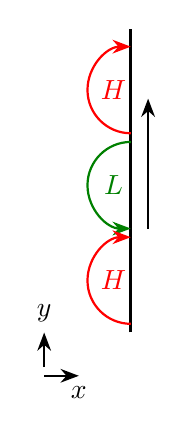
\begin{tikzpicture}[scale=1.1, >=Stealth]

    % draw the sidewall going up/down:

    \draw[very thick] (1,0) -- (1,3.5) node[midway, right] {};

    % Draw a curve that goes from y=1.2 to 1.7 and out as far as 0.7

    \draw[thick, darkgreen, <-] (1,1.2) arc[start angle=270, end angle=90, radius=0.5];
    \node[text=darkgreen] at (0.8,1.7) {$L$};

    \draw[thick, red, ->] (1,2.3) arc[start angle=270, end angle=90, radius=0.5];
    \node[text=red] at (0.8,2.8) {$H$};

    \draw[thick, red, ->] (1,0.1) arc[start angle=270, end angle=90, radius=0.5];
    \node[text=red] at (0.8,0.6) {$H$};

    \draw[thick, black, ->] (1.2,1.2) -- (1.2, 2.7);

    % small axes indicating x and y directions:
    \draw[->, thick] (0,-0.5) -- (0.4,-0.5) node[below] {$x$};
    \draw[->, thick] (0,-0.40) -- (0,0.0) node[above] {$y$};
%
\end{tikzpicture}
\end{document}
